% Wczytanie szablonu
\documentclass[nostrict]{Szablon}

% Definicja dokumentu
\usepackage[unicode=true]{hyperref}
\usepackage{listings}
\usepackage{xcolor}
% Allow [H] placement for floats (tables/figures)
\usepackage{float}


% Konfiguracja dla listings
\lstset{
    basicstyle=\ttfamily\small,
    backgroundcolor=\color{gray!10},
    frame=single,
    breaklines=true,
    captionpos=b
}

\newcommand\PDFtitle{Tytuł pracy}
\newcommand\PDFauthors{Filip Jezierski, Michał Pawiłojć, Michał Turski, Karina Wołoszyn}
\hypersetup{
  pdftitle={\PDFtitle},
  pdfauthor={\PDFauthors},
}
    
% Zmiana czcionki dla symulacji maszynopisu (verbatim)
\makeatletter
\renewcommand{\verbatim@font}{\ttfamily\small}
\makeatother

% Część właściwa pracy
\begin{document}
\chapter*{Streszczenie}
%\addcontentsline{toc}{chapter}{Streszczenie}  
Niniejsza praca prezentuje opracowanie aplikacji mobilnej typu PWA, która umożliwia interaktywną rozgrywkę polegającą na odgadywaniu lokalizacji na podstawie zdjęć oraz weryfikowaniu obecności w wybranych miejscach z wykorzystaniem geolokalizacji. Praca rozpoczyna się od analizy sytuacji na rynku i uzasadnienia wyboru tematu, a następnie przedstawia szczegółowy podział prac oraz wprowadzenie do dziedziny aplikacji mobilnych i gier edukacyjno-rozrywkowych.

W pracy omówiono technologie i narzędzia wykorzystane w projekcie, w tym frameworki frontendowe i backendowe, systemy mapowe oraz mechanizmy geolokalizacji. Na podstawie analizy wymagań użytkowych i systemowych zaprojektowano architekturę aplikacji, uwzględniając zarówno aspekt funkcjonalny, jak i niefunkcjonalny, w tym responsywność, estetykę interfejsu i wydajność.

Część implementacyjna obejmuje szczegółowy opis tworzenia frontendu i backendu, integrację z usługami zewnętrznymi oraz implementację mechanizmów rozgrywki, takich jak tryby klasyczny i geolokalizacyjny, system punktacji, historia rozgrywek i ranking użytkowników. W pracy przedstawiono także konfigurację aplikacji PWA, zarządzanie sesjami użytkowników oraz obsługę zdjęć lokalizacji.

Rozdział dotyczący testowania opisuje przeprowadzone testy manualne funkcjonalności oraz weryfikację stabilności i poprawności działania aplikacji na różnych urządzeniach i przeglądarkach. W podsumowaniu pracy omówiono osiągnięte cele oraz wskazano potencjalne kierunki dalszego rozwoju projektu, takie jak rozbudowa bazy lokalizacji, wprowadzenie nowych trybów gry czy integracja z dodatkowymi usługami sieciowymi.

Praca przedstawia pełen proces projektowania, implementacji i testowania aplikacji mobilnej typu PWA, łączącej funkcjonalności edukacyjne i rozrywkowe w intuicyjnym i atrakcyjnym interfejsie użytkownika.

\chapter*{Abstract}
%\addcontentsline{toc}{chapter}{Abstract}
This thesis presents the development of a mobile PWA application that enables interactive gameplay based on guessing locations from photos and verifying presence in selected places using geolocation. The work begins with a market analysis and justification for the topic choice, followed by a detailed work distribution and an introduction to the field of mobile applications and educational-entertainment games.

The thesis discusses the technologies and tools used in the project, including frontend and backend frameworks, mapping systems, and geolocation mechanisms. Based on the analysis of user and system requirements, the application architecture was designed, considering both functional and non-functional aspects, including responsiveness, interface aesthetics, and performance.

The implementation section includes a detailed description of frontend and backend development, integration with external services, and the implementation of gameplay mechanisms such as classic and geolocation modes, scoring system, game history, and user ranking. The thesis also presents the configuration of the PWA application, user session management, and photo handling for locations.

The testing chapter describes the manual functional tests conducted and the verification of the application's stability and correctness across different devices and browsers. In the conclusion, the achieved goals are discussed, and potential directions for further project development are indicated, such as expanding the location database, introducing new game modes, or integrating with additional web services.

The thesis presents the complete process of designing, implementing, and testing a mobile PWA application that combines educational and entertainment functionalities in an intuitive and attractive user interface.

\include{chapters/0b_spis_tresci}
\chapter*{Wykaz ważniejszych oznaczeń i skrótów}
\addcontentsline{toc}{chapter}{Wykaz ważniejszych oznaczeń i skrótów}

\begin{itemize}
  \item \textbf{API} (ang. \textit{Application Programming Interface}) - zestaw reguł i protokołów określających sposób komunikacji oraz integracji pomiędzy różnymi elementami aplikacji.
  \item \textbf{AR} (ang. \textit{Augmented Reality}) - technologia rozszerzonej rzeczywistości, która łączy elementy wirtualne z rzeczywistym światem użytkownika.
  \item \textbf{CI/CD} (ang. \textit{Continuous Integration / Continuous Delivery lub Deployment}) - zestaw praktyk automatyzujących budowanie, testowanie i dostarczanie oprogramowania, dzięki czemu zmiany trafiają do użytkowników szybciej i bardziej niezawodnie.
  \item \textbf{CORS} (ang. \textit{Cross-Origin Resource Sharing}) - mechanizm kontrolujący, które domeny mogą wykonywać zapytania do zasobów serwera.
  \item \textbf{CQRS} (ang. \textit{Command Query Responsibility Segregation}) - wzorzec architektoniczny polegający na rozdzieleniu operacji modyfikujących stan systemu od operacji odczytujących dane.
  \item \textbf{DDD} (ang. \textit{Domain-Driven Design}) - podejście do projektowania oprogramowania, które skupia sie na odwzorowywaniu rzeczywistego świata w modelu domeny.
  \item \textbf{DOM} (ang. \textit{Document Object Model}) - struktura reprezentująca dokumenty HTML i XML jako hierarchię obiektów, umożliwiająca manipulację ich zawartością i strukturą za pomocą języków programowania.
  \item \textbf{DTO} (ang. \textit{Data Transfer Object}) - obiekt służący do przenoszenia danych między warstwami aplikacji.
  \item \textbf{E2E} (ang. \textit{End-to-End}) - rodzaj testów sprawdzających cały przepływ działania aplikacji z perspektywy użytkownika.
  \item \textbf{ERD} (ang. \textit{Entity-Relationship Diagram}) - diagram związków encji, służący do modelowania struktury bazy danych.
  \item \textbf{GPS} (ang. \textit{Global Positioning System}) - system nawigacji satelitarnej umożliwiający określenie położenia geograficznego na powierzchni Ziemi.
  \item \textbf{GUI} (ang. \textit{Graphical User Interface}) - graficzny interfejs użytkownika oparty na elementach wizualnych, takich jak okna, ikony czy przyciski.
  \item \textbf{HTML} (ang. \textit{HyperText Markup Language}) - język znaczników używany do tworzenia stron internetowych.
  \item \textbf{HSTS} (ang. \textit{HTTP Strict Transport Security}) - mechanizm wymuszający użycie HTTPS, chroniący przed atakami typu downgrading i przechwytywaniem sesji.
  \item \textbf{HTTP} (ang. \textit{HyperText Transfer Protocol}) - podstawowy protokół komunikacji w sieci WWW, umożliwiający przesyłanie stron internetowych oraz danych między klientem a serwerem.
  \item \textbf{HTTPS} (ang. \textit{HyperText Transfer Protocol Secure}) - bezpieczna wersja protokołu HTTP, która wykorzystuje szyfrowanie SSL/TLS do ochrony przesyłanych danych.
  \item \textbf{IDE} (ang. \textit{Integrated Development Environment}) - zintegrowane środowisko programistyczne zawierające narzędzia potrzebne do tworzenia i debugowania kodu.
  \item \textbf{ITS} (ang. \textit{Issue Tracker System}) - sposób zarządzania systemem, który odpowiada na zapytania wysyłane dowolną drogą.
  \item \textbf{JSON} (ang. \textit{JavaScript Object Notation}) - format wymiany danych oparty na składni języka JavaScript.
  \item \textbf{JWT} (ang. \textit{JSON Web Token}) - standardowy format bezpiecznego przesyłania informacji jako obiekt JSON.
  \item \textbf{LINQ} (ang. \textit{Language Integrated Query}) - zestaw technik umożliwiających tworzenie zapytań bezpośrednio w kodzie C\#, w spójny sposób niezależnie od źródła danych.
  \item \textbf{NPM} (ang. \textit{Node Package Manager}) - manager pakietów dedykowany środowisku Node.js.
  \item \textbf{ORM} (ang. \textit{Object-Relational Mapping}) - technika mapowania danych między systemem obiektowym a relacyjną bazą danych.
  \item \textbf{PWA} (ang. \textit{Progressive Web Application}) - aplikacja webowa wykorzystująca nowoczesne technologie webowe w celu zapewnienia doświadczenia podobnego do aplikacji natywnych.
  \item \textbf{QA} (ang. \textit{Quality Assurance}) - zestaw procesów i praktyk mających zapewnić wysoką jakość tworzonego oprogramowania.
  \item \textbf{REST} (ang. \textit{Representational State Transfer}) - styl architektoniczny wykorzystywany przy projektowaniu usług sieciowych.
  \item \textbf{SQL} (ang. \textit{Structured Query Language}) - strukturalny język zapytań służący do definiowania, modyfikowania i pobierania danych z relacyjnych baz danych.
  \item \textbf{TLS} (ang. \textit{Transport Layer Security}) - protokół szyfrujący zapewniający poufność i integralność danych przesyłanych w sieci.
  \item \textbf{UI} (ang. \textit{User Interface}) - interfejs użytkownika, czyli sposób prezentacji i organizacji elementów umożliwiających interakcję z aplikacją.
  \item \textbf{UX} (ang. \textit{User Experience}) - doświadczenie użytkownika obejmujące wrażenia, odczucia i wygodę korzystania z produktu lub systemu.
  \item \textbf{WWW} (ang. \textit{World Wide Web}) - system zasobów internetowych połączonych hiperłączami, umożliwiający przeglądanie stron i treści za pomocą przeglądarki.
  \item \textbf{VCS} (ang. \textit{Version Control System}) - system kontroli wersji pozwalający śledzić zmiany w kodzie, zarządzać historią projektu i pracą zespołową.
  \item \textbf{VM} (ang. \textit{Virtual Machine}) - maszyna wirtualna emulująca komputer w celu uruchamiania systemów operacyjnych lub aplikacji w izolowanym środowisku.
  \item \textbf{VS} (ang. \textit{Visual Studio}) - zintegrowane środowisko programistyczne (IDE) stworzone przez firmę Microsoft
  \item \textbf{YAML} (ang. \textit{YAML Ain't Markup Language}) - lekki format plików konfiguracyjnych oparty na strukturze wcięć.
\end{itemize}

\chapter{Wstęp i cel pracy}
\label{chap:introduction}

Celem projektu jest stworzenie gry geograficzno-geolokalizacyjnej polegającej na odgadywaniu miejsc związanych z Politechniką Gdańską na podstawie ich zdjęć. Dodatkowo dostępny będzie tryb terenowy, w którym użytkownik musi fizycznie udać się w odgadywane miejsce. Aby zwiększyć stopień interakcji między użytkownikami, zaplanowaliśmy również udostępnienie publicznego rankingu, zachęcającego do poprawiania swoich wyników, a także dodanie trybu wieloosobowego, w którym gracze rywalizowaliby między sobą, ścigając się o to, kto pierwszy odgadnie zadaną lokalizację.

Aplikacja taka pozwalałaby na interaktywne poznawanie terenów kampusu dla szerokiego grona zainteresowanych, od osób niezwiązanych z uczelnią, do absolwentów oraz pracowników PG. Szczególnie przydatnym zastosowaniem byłoby zapoznawanie przyszłych i nowych studentów z okolicami uczelni, ułatwiając im orientację w nowym otoczeniu.

Gry przeglądarkowe cieszyły się popularnością od momentu ich powstania. Ich głównym atutem są niskie wymagania sprzętowe czy brak potrzeby instalacji, które od początku poszerzyły grono potencjalnych odbiorców. Dodatkowo, użytkownicy za pośrednictwem dostępu do internetu mogą wchodzić ze sobą w interakcje i rywalizować dzięki udostępnianym rankingom.

Popularność gier komputerowych znacząco wzrosła podczas pandemii COVID-19, gdzie przez potrzebę pozostania w izolacji możliwości spędzania wolnego czasu były ograniczone. Wydłużony czas pozostania w domach przyczynił się też do wzrostu zainteresowania grami geograficznymi i geolokalizacyjnymi. Jednym z czołowych produktów tego zjawiska został GeoGuessr, który mimo wypuszczenia na rynek 6 lat wcześniej, został spopularyzowany dopiero w 2020 roku. Sukces ten można przypisać idei połączenia rozrywki i odkrywania świata z wykorzystaniem Google Street View, dzięki której użytkownicy mogą się wykazać wiedzą na temat architektury, ukształtowania terenu oraz panującego w danym kraju języka.

Podobnym trendem wykazały się aplikacje mobilne, które ze względu na szybki rozwój urządzeń przenośnych, pozwalają graczowi połączyć się z dowolnego miejsca, w dowolnej chwili. Zlikwidowały one potrzebę posiadania drogiego i nieporęcznego sprzętu, stawiając na wygodę użytkownika. Atuty te wykorzystała gra Pokemon Go, która z pomocą dobrze znanej marki podbiła rynek, osiągając pułap 500 milionów pobrań w pierwszym roku po debiucie. Gra ta korzysta z funkcji GPS do znalezienia wirtualnych aren rozsianych po prawdziwych lokalizacjach, przyczyniając się do zwiększenia immersji rozgrywki.

Po dokonaniu powyższej analizy rynku, postanowiliśmy w ramach projektu inżynierskiego stworzyć aplikację łączącą w sobie dotychczas wymienione aspekty.
 % cel pracy, motywacja, sytuacja na rynku
\chapter{Wprowadzenie do dziedziny}
\label{chap:field}

\section{Rynek gier przeglądarkowych}

\section{Rynek gier geolokalizacyjnych}

\section{Rodzaje gier konkurencyjnych}

\include{chapters/3_wykorzystane_technologie}
\include{chapters/4_narzedzia}
\chapter{Analiza wymagań}
\label{chap:algs}

\section{Koncepcja gry}
\section{Przebieg gry}
\section{Tryby rozgrywki}
\section{Wymagania funkcjonalne}

\section{Wymagania niefunkcjonalne (Filip Jezierski)}
Wymagania niefunkcjonalne określają kryteria jakościowe, które aplikacja powinna spełniać, aby zapewnić odpowiednie doświadczenie użytkownika oraz efektywne działanie systemu. W kontekście opracowywanej aplikacji mobilnej, kluczowe wymagania niefunkcjonalne obejmują aspekty takie jak wydajność, bezpieczeństwo oraz użyteczność.

\subsection{Wymagania jakościowe}
\begin{itemize}
    \item obsługa różnych rozdzielczości ekranów i urządzeń mobilnych,
    \item dostępność aplikacji na popularnych platformach mobilnych (Android, iOS), a także jako aplikacja webowa,
    \item intuicyjny i responsywny interfejs użytkownika,
    \item aplikacja powinna w odpowiedni sposób obsługiwać błędy i wyjątki, takie jak nieprawidłowe dane wejściowe czy brak internetu, zapewniając stabilność działania,
    \item ochrona danych użytkowników poprzez implementację odpowiednich mechanizmów bezpieczeństwa - szyfrowanie danych, bezpieczne logowanie, ochrona przed atakami typu SQL Injection i XSS.
\end{itemize}

\subsection{Wymagania wydajnościowe}
\begin{itemize}
    \item szybkie (<2 s) ładowanie aplikacji i minimalny czas oczekiwania na reakcję interfejsu użytkownika,
    \item ładowanie zdjęć lokalizacji w czasie nie dłuższym niż 3 sekundy,
    \item szybkie (<10 s) ładowanie danych geolokalizacyjnych zapewniające płynne działanie trybu gry opartego na lokalizacji,
\end{itemize}

\section{Wybór platformy (Filip Jezierski)}
Wybór odpowiedniej platformy dla opracowywanej aplikacji mobilnej jest kluczowym elementem procesu projektowego, mającym istotny wpływ na jej funkcjonalność, dostępność oraz doświadczenie użytkownika, a także łatwość wdrożenia i utrzymania. Na etapie analizy wymagań podjęto decyzję o stworzeniu dwóch testowych wersji aplikacji: aplikacji webowej typu PWA (Progressive Web App) oraz natywnej aplikacji mobilnej wykorzystującej technologię .NET MAUI (Multi-platform App UI). Obie platformy oferują unikalne korzyści i wyzwania, które zostały dokładnie rozważone w kontekście specyfiki projektu.

\subsection{Natywna aplikacja mobilna}
Aplikacje natywne są tworzone z wykorzystaniem dedykowanych narzędzi i języków programowania przeznaczonych dla konkretnych systemów operacyjnych, takich jak Android czy iOS. W przypadku technologii .NET MAUI możliwe jest tworzenie aplikacji wieloplatformowych przy zachowaniu wspólnej bazy kodu, co znacząco skraca czas implementacji i ułatwia utrzymanie.

Jednakże proces publikacji aplikacji natywnych w sklepach takich jak Google Play czy Apple App Store wiąże się z dodatkowymi wymaganiami i procedurami zatwierdzania, a także z koniecznością budowania i testowania aplikacji na różne systemy operacyjne, co może wydłużyć czas wdrożenia.

\subsection{Aplikacja webowa PWA}
Aplikacja webowa typu PWA (Progressive Web App) łączy cechy klasycznej strony internetowej z funkcjonalnością aplikacji mobilnej. Dzięki wykorzystaniu nowoczesnych technologii webowych, możliwe jest stworzenie aplikacji działającej w trybie offline, instalowanej bezpośrednio z przeglądarki oraz zapewniającej wrażenia zbliżone do aplikacji natywnej.

Ze względu na łatwość dostępu (poprzez przeglądarkę internetową) oraz brak konieczności przechodzenia przez proces zatwierdzania w sklepach aplikacji, PWA stanowi atrakcyjną opcję dla naszego projektu. Jednakże, pewne ograniczenia związane z dostępem do funkcji urządzenia (takich jak geolokalizacja) oraz wydajnością w porównaniu do aplikacji natywnych muszą być uwzględnione podczas projektowania i implementacji.

\section{Ograniczenia projektu (Filip Jezierski)}
Ograniczenia projektu wynikają przede wszystkim z przyjętych założeń technologicznych oraz charakteru opracowywanego rozwiązania. Kluczowe znaczenie mają tu specyfika aplikacji webowej typu PWA, zastosowanie mechanizmów geolokalizacji jako podstawowego elementu funkcjonalnego, a także decyzje dotyczące sposobu pozyskiwania i wykorzystania materiałów wizualnych. Wymienione czynniki w naturalny sposób wpływają na zakres możliwości implementacyjnych, wydajność rozwiązania oraz doświadczenie użytkownika końcowego.

\subsection{Środowisko aplikacji}
Aplikacja będzie udostępniana jako aplikacja webowa, dostępna przez przeglądarkę internetową, z możliwością instalacji na ekranie głównym urządzenia. Funkcjonalność trybu gry wykorzystującego geolokalizację będzie dostępna wyłącznie na urządzeniach mobilnych, które wspierają tę technologię. W przypadku urządzeń stacjonarnych, nawet jeśli geolokalizacja jest technicznie możliwa, jej dokładność jest niewystarczająca do zapewnienia poprawnego działania tej funkcji.

\subsection{Zdjęcia lokalizacji}
W projekcie zrezygnowano z wykorzystywania zdjęć 360° pochodzących z zewnętrznych źródeł, takich jak interfejsy API udostępniane przez firmy trzecie. Decyzję tę podjęto z uwagi na chęć uniknięcia potencjalnych problemów związanych z licencjonowaniem, ograniczoną dostępnością materiałów oraz zróżnicowaną jakością zdjęć. Dodatkowo korzystanie z takich źródeł mogłoby wprowadzać ograniczenia dotyczące liczby i różnorodności dostępnych lokalizacji.

W celu uproszczenia procesu pozyskiwania materiałów wizualnych oraz umożliwienia użytkownikom współtworzenia bazy lokalizacji, aplikacja będzie wykorzystywać standardowe zdjęcia dwuwymiarowe. Tego typu fotografie nie wymagają specjalistycznego sprzętu i mogą być wykonywane przy użyciu dowolnego smartfona. Użytkownicy będą mieli możliwość przesyłania własnych zdjęć lokalizacji, które po weryfikacji przez moderatorów zostaną dodane do bazy danych aplikacji.

Takie rozwiązanie zapewnia pełną kontrolę nad jakością i zgodnością materiałów z założeniami projektu, a jednocześnie pozwala na stopniowe rozszerzanie bazy lokalizacji o nowe zdjęcia, dostarczane zarówno przez zespół projektowy, jak i społeczność użytkowników.

\section{Kryteria akceptacji (Filip Jezierski)}
\textbf{Ogólne kryteria:}
\begin{itemize}
    \item Aplikacja działa na urządzeniach mobilnych z systemami Android i iOS, na komputerach stacjonarnych oraz w przeglądarkach internetowych
    \item Intuicyjny interfejs użytkownika umożliwiający łatwe korzystanie z aplikacji
    \item Responsywny design dostosowujący się do różnych rozmiarów ekranów, w szczególności urządzeń mobilnych
    \item Stabilne działanie aplikacji bez krytycznych błędów i awarii
    \item Testy manualne wszystkich zaplanowanych funkcjonalności przeprowadzone na wszystkich wspieranych platformach
\end{itemize}

\textbf{Zaimplementowane funkcjonalności:}
\begin{itemize}
    \item Rejestracja i logowanie użytkowników
    \item Wybór trybu rozgrywki i poziomu trudności
    \item Dwa tryby gry:
    \begin{itemize}
        \item odgadywanie lokalizacji na podstawie zdjęcia poprzez wskazanie jej na mapie
        \item odnajdywanie lokalizacji na podstawie zdjęcia i potwierdzanie obecności poprzez geolokalizację
    \end{itemize}
    \item Możliwość przerywania i kontynuowania rozgrywki
    \item Wyświetlanie podsumowania wyników każdej rundy gry
    \item Historia rozgrywek dostępna w profilu użytkownika
    \item Ogólnodostępny ranking graczy
    \item Dodawanie lokalizacji przez użytkowników (po weryfikacji przez moderatorów)
\end{itemize}

\chapter{Projekt systemu (Michał Turski i Filip Jezierski)}
\label{chap:system_project}
Niniejszy rozdział przedstawia szczegółowy projekt systemu aplikacji webowej \textbf{UniGuesser}. Opisane zostaną kluczowe elementy architektury systemu, w tym warstwy aplikacji, baza danych oraz najbardziej kluczowe interakcje użytkownika z systemem. Zaczynając od ogólnego przeglądu architektury, przejdziemy do szczegółowego omówienia poszczególnych komponentów i ich wzajemnych relacji.

W aplikacji zastosowano architekturę warstwową, której szczegółowa implementacja zostanie opisana w niniejszym rozdziale. Na najwyższym poziomie abstrakcji system można podzielić na trzy główne warstwy: warstwę prezentacji (frontend), warstwę logiki biznesowej (backend) oraz warstwę persystencji danych (baza danych). Podział ten odzwierciedla sposób izolowania odpowiedzialności poszczególnych komponentów. Dzięki temu użytkownik komunikuje się z aplikacją poprzez interfejs użytkownika, który następnie przekazuje żądania do warstwy logiki biznesowej. Ta z kolei przetwarza żądania, wykonuje odpowiednie operacje i komunikuje się z bazą danych w celu przechowywania lub pobierania danych.

\begin{figure}[h]
    \centering
    
\includegraphics[width=1.0\textwidth]{./images/architecture-overview.png}
    \caption{Uproszczony schemat architektury systemu UniGuesser – ogólny podział na warstwy}
    \label{fig:architecture-overview}
\end{figure}


\section{Architektura logiki biznesowej (Michał Turski)}
Architektura w aplikacji \textbf{UniGuesser} została zbudowana w oparciu o Command-Query Responsibility Segregation (CQRS) oraz Domain-Driven Design (DDD), które
są obecnie standardem w wytwarzaniu oprogramowania. [dodać źródło na potwierdznie słów]
Ponadto zdecydowaliśmy na wybór architektury monolitycznej ze względu na szybkość rozwoju i łatwość wdrożenia, co pomogło skupić się nam na aspekcie funkcjonalnym aplikacji w początkowej fazie jej tworzenia.

\subsection{Wzorzec CQRS (Command Query Responsibility Segregation)}
Wykorzystany został również wzorzec CQRS. Zakłada on rozdzielenie operacji modyfikujących stan systemu (komendy) od operacji, które odczytują dane (zapytania). Pozwala to na lepsze skalowanie i rozdzielenie logiki aplikacji. Dzięki temu można optymalizować każdą z tych operacji niezależnie, co przekłada się na wydajność i czytelność kodu. W kontekście skalowalności systemu zastosowano uproszczoną implementację wzorca CQRS z pojedynczą bazą danych, która jest wystarczająca przy przewidywanym obciążeniu nieprzekraczającym 50 zapytań na sekundę. Taka architektura zapewnia odpowiednią wydajność przy jednoczesnym zachowaniu prostoty infrastruktury.

\begin{figure}[h]
    \centering
    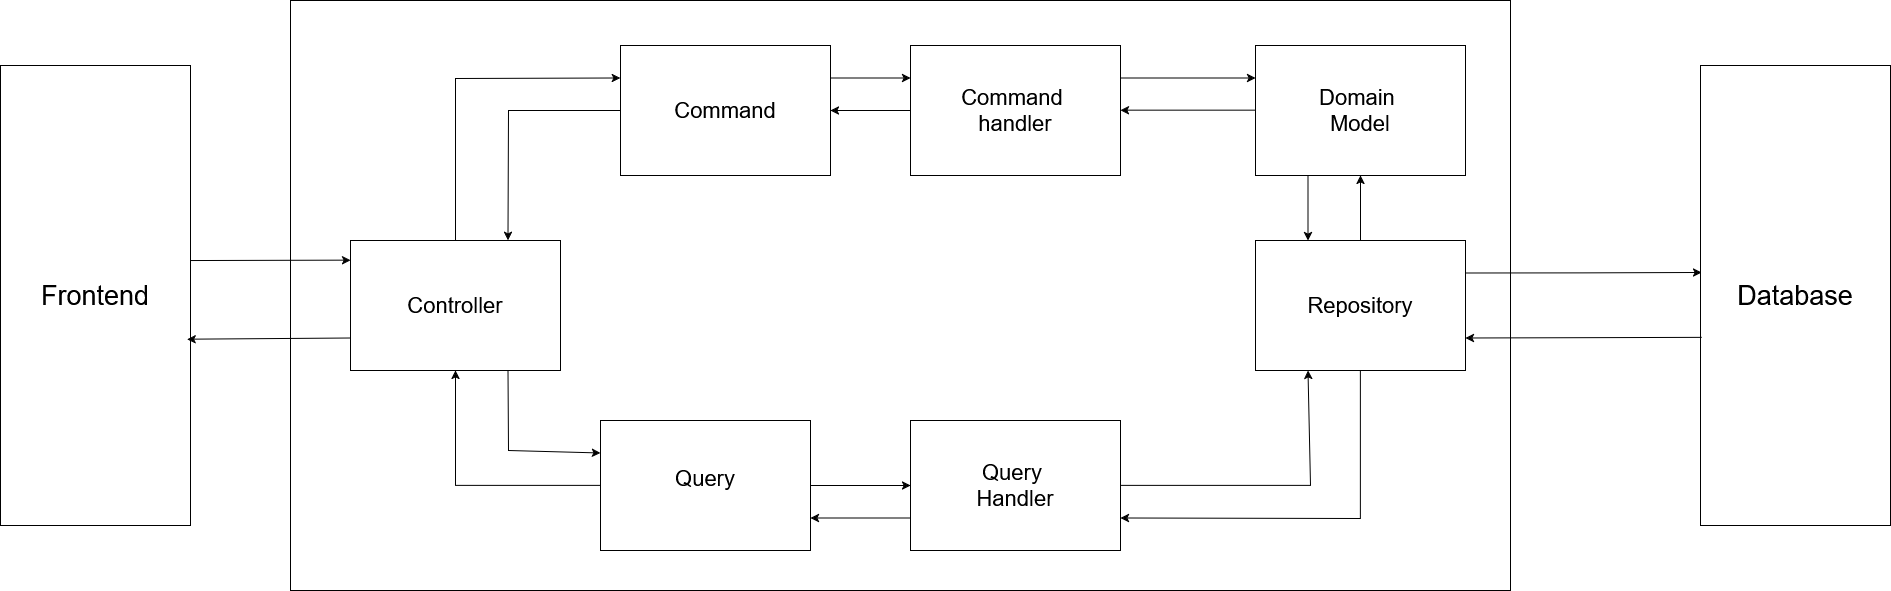
\includegraphics[width=1.0\textwidth]{./images/cqrs-communication.png}
    \caption{Schemat komunikacji przy zastosowaniu wzorca CQRS}
    \label{fig:cqrs-communication}
\end{figure}



\subsection{Zastosowanie DDD (Domain-Driven Design)}
Model systemu został zaprojektowany zgodnie z podejściem Domain-Driven Design (DDD), które kładzie nacisk na zrozumienie i modelowanie domeny problemowej. W aplikacji definiujemy trzy główne warstwy DDD: warstwę domeny, warstwę aplikacji oraz warstwę infrastruktury. Każda z warstw znajduje się w osobnym module, co ułatwia zarządzanie kodem i jego rozwój. Dodatkowo w aplikacji wydzielony został czwarty moduł „API”, który odpowiada za komunikację z warstwą prezentacji, co zmniejsza złożoność warstwy aplikacji. Moduł „API” obsługuje zarówno zapytania, jak i komendy, delegując je odpowiednio do warstwy aplikacji, która następnie komunikuje się z warstwą domeny i infrastruktury w celu realizacji żądanych operacji.

\section{Baza danych (Michał Turski)}

W aplikacji zastosowano relacyjną bazę danych, do przechowywania informacji o aktualnych i przeszłych sesjach gier, użytkownikach, lokalizacjach oraz wynikach. Zdecydowaliśmy się na wykorzystanie relacyjnej bazy danych ze względu na duża ilość powiąza między encjami oraz potrzebę zapewnienia integralności danych między nimi. Relacyjne bazy danych zapewniaja ACID (Atomicity, Consistency, Isolation, Durability), co jest kluczowe dla zachowania spójności danych w rozgrywce. 

\subsection{Diagram ERD}
Przedstawiony na rysunku \ref{fig:erd-diagram} diagram ERD (Entity-Relationship Diagram) ilustruje strukturę bazy danych aplikacji UniGuesser, pokazując główne tabele oraz relacje między nimi. Użytkownik może posiadać wiele sesji gier, a każda sesja ma określoną liczbę rund, z których każda posiada przypisaną do siebie lokacje. Ponadto każde miejsce może mieć swojego autora (użytkownika), który dodał je do bazy danych. 

\begin{figure}[h]
    \centering
    
\includegraphics[width=1.0\textwidth]{./images/erdDiagram.png}
    \caption{Diagram ERD (Entity-Relationship Diagram) dla bazy danych aplikacji UniGuesser}
    \label{fig:erd-diagram}
\end{figure}

\subsection{Opis głównych tabel i związków}

\begin{itemize}
    \item \textbf{Users (Użytkownicy)} – tabela przechowująca informacje o użytkownikach aplikacji.
\end{itemize}

\begin{table}[H]
\centering
\renewcommand{\arraystretch}{1.2}
\begin{tabular}{|p{2.5cm}|p{8cm}|p{2.5cm}|}
\hline
\textbf{Atrybut} & \textbf{Opis} & \textbf{Typ / Uwagi} \\ \hline
ID & Unikalny identyfikator użytkownika. & Klucz główny \\ \hline
Nickname & Unikalna nazwa użytkownika. & Tekst \\ \hline
Email & Unikalny adres e-mail użytkownika. & Tekst \\ \hline
PasswordHash & Zaszyfrowane hasło użytkownika. & Tekst \\ \hline
CreatedAt & Data i czas utworzenia konta. & Data/Czas \\ \hline
Role & Rola użytkownika w systemie (np. użytkownik, administrator). & Enumeracja \\ \hline
\end{tabular}
\caption{Tabela \texttt{Users}}

\end{table}

\textbf{GameSessions (Sesje gier)} – tabela przechowująca informacje o aktywnych i zakończonych rozgrywkach.

\begin{table}[H]
\centering
\renewcommand{\arraystretch}{1.2}
\begin{tabular}{|p{2.8cm}|p{8.5cm}|p{2cm}|}
\hline
\textbf{Atrybut} & \textbf{Opis} & \textbf{Typ / Uwagi} \\ \hline
ID & Unikalny identyfikator sesji gry. & Klucz główny \\ \hline
GameMode & Tryb gry w danej sesji. & Enumeracja \\ \hline
GameEndDate & Data, do której rozgrywka jest aktywna. & Data/Czas \\ \hline
RoundNumber & Aktualnie rozgrywana runda. & Liczba \\ \hline
GameScore & Łączna liczba punktów zdobytych. & Liczba całkowita \\ \hline
Difficulty & Poziom trudności sesji. & Enumeracja \\ \hline
FinishedTime & Data zakończenia rozgrywki. & Data/Czas \\ \hline
UserID & Identyfikator użytkownika. & Klucz obcy → Users \\ \hline
\end{tabular}
\caption{Tabela \texttt{GameSessions}}
\label{tab:game-sessions}
\end{table}

\textbf{Rounds (Rundy)} – tabela przechowująca informacje o poszczególnych rundach w sesji gry.

\begin{table}[H]
\centering
\renewcommand{\arraystretch}{1.2}
\begin{tabular}{|p{3cm}|p{8.5cm}|p{1.8cm}|}
\hline
\textbf{Atrybut} & \textbf{Opis} & \textbf{Typ / Uwagi} \\ \hline
ID & Unikalny identyfikator rundy. & Klucz główny \\ \hline
GuessedLatitude & Szerokość geograficzna wskazana przez użytkownika. & Liczba zmiennoprzecinkowa \\ \hline
GuessedLongitude & Długość geograficzna wskazana przez użytkownika. & Liczba zmiennoprzecinkowa \\ \hline
Score & Punkty zdobyte w rundzie. & Liczba całkowita \\ \hline
GameSessionID & Identyfikator sesji gry. & Klucz obcy → GameSessions \\ \hline
LocationID & Identyfikator lokacji. & Klucz obcy → Places \\ \hline
\end{tabular}
\caption{Tabela \texttt{Rounds}} 
\label{tab:rounds}
\end{table}

\textbf{Places (Lokacje)} – tabela przechowująca informacje o lokacjach dostępnych w grze.

\begin{table}[H]
\centering
\renewcommand{\arraystretch}{1.2}
\begin{tabular}{|p{2.5cm}|p{8cm}|p{2.5cm}|}
\hline
\textbf{Atrybut} & \textbf{Opis} & \textbf{Typ / Uwagi} \\ \hline
ID & Unikalny identyfikator lokacji. & Klucz główny \\ \hline
Name & Nazwa lokacji. & Tekst \\ \hline
Description & Opis lokacji. & Tekst \\ \hline
Latitude & Szerokość geograficzna lokacji. & Liczba zmiennoprzecinkowa \\ \hline
Longitude & Długość geograficzna lokacji. & Liczba zmiennoprzecinkowa \\ \hline
Difficulty & Poziom trudności lokacji. & Enumeracja \\ \hline
ImageUrl & Adres URL obrazu lokacji. & Tekst \\ \hline
AltImage & Tekst alternatywny dla obrazu lokacji. & Tekst \\ \hline
CreationTime & Data i czas dodania lokacji. & Data/Czas \\ \hline
AuthorID & Identyfikator autora lokacji. & Klucz obcy → Users \\ \hline
\end{tabular}
\caption{Tabela \texttt{Places}}
\end{table}

\section{Analiza interakcji użytkownika z systemem (Michał Turski)}
W rozdziale przedstawione zostaną możliwości i przebieg kluczowych funkcjonalności aplikacji UniGuesser z perspektywy użytkownika końcowego. Opisane zostaną główne przypadki użycia oraz interakcje między użytkownikiem a systemem podczas typowej rozgrywki.

\subsection{Przypadki użycia aplikacji}
Przedstawiony na rysunku \ref{fig:use-case-diagram} diagram przypadków użycia ilustruje główne funkcjonalności aplikacji UniGuesser z perspektywy użytkownika moderatora i administratora. Użytkownik może rejestrować się i logować do systemu, rozpoczynać nowe sesje gier, uczestniczyć w rozgrywkach, przeglądać wyniki innych użytkowników, oraz proponować nowe lokacje. Moderator dodatkowo może zatwierdzać lub odrzucać proponowane lokacje, natomiast administrator ma uprawnienia do zarządzania użytkownikami.

\begin{figure}[H]
    \centering
    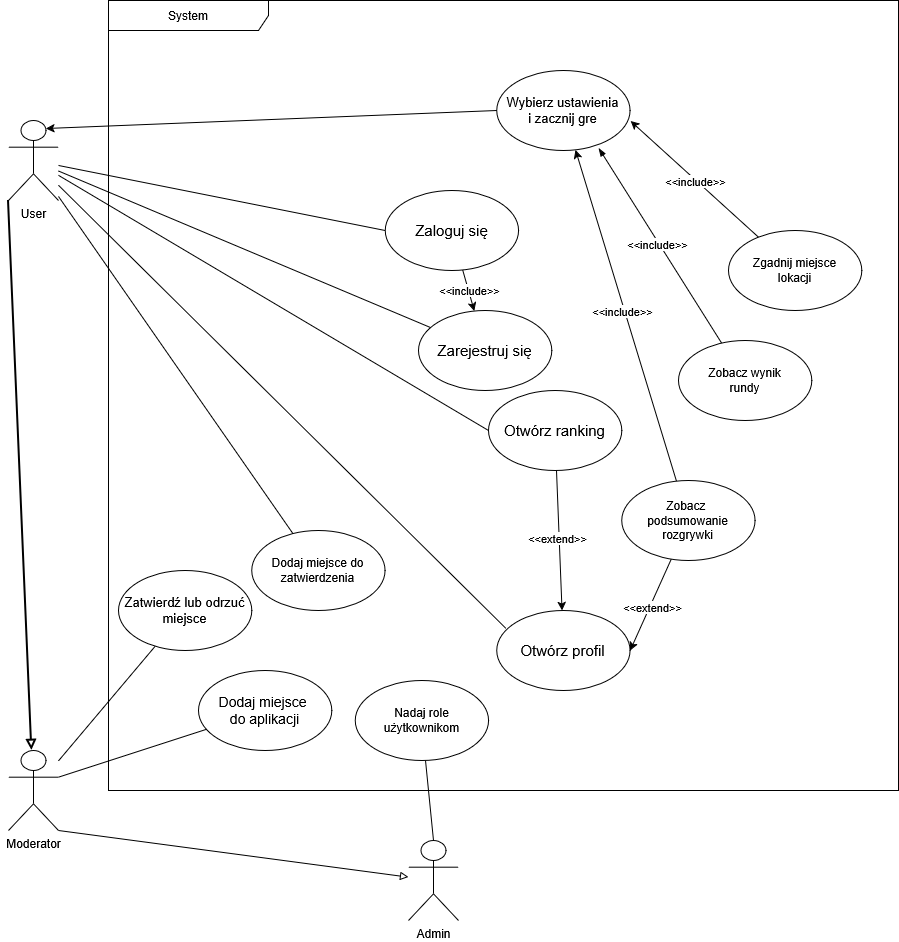
\includegraphics[width=1.0\textwidth]{./images/useCaseDiagram.png}
    \caption{Diagram przypadków użycia aplikacji UniGuesser}
    \label{fig:use-case-diagram}
\end{figure}

\subsection{Diagram sekwencji rozgrywki}

Diagram sekwencji przedstawiony na rysunku \ref{fig:sequence-diagram} ilustruje przebieg interakcji między użytkownikiem a systemem podczas typowej rozgrywki w aplikacji UniGuesser. Proces rozpoczyna się od momentu, gdy użytkownik uruchamia nową grę, poprzez kolejne rundy, aż do momentu zakończenia sesji i wyświetlenia wyników końcowych.

\begin{figure}[H]
    \centering
    \makebox[\textwidth]{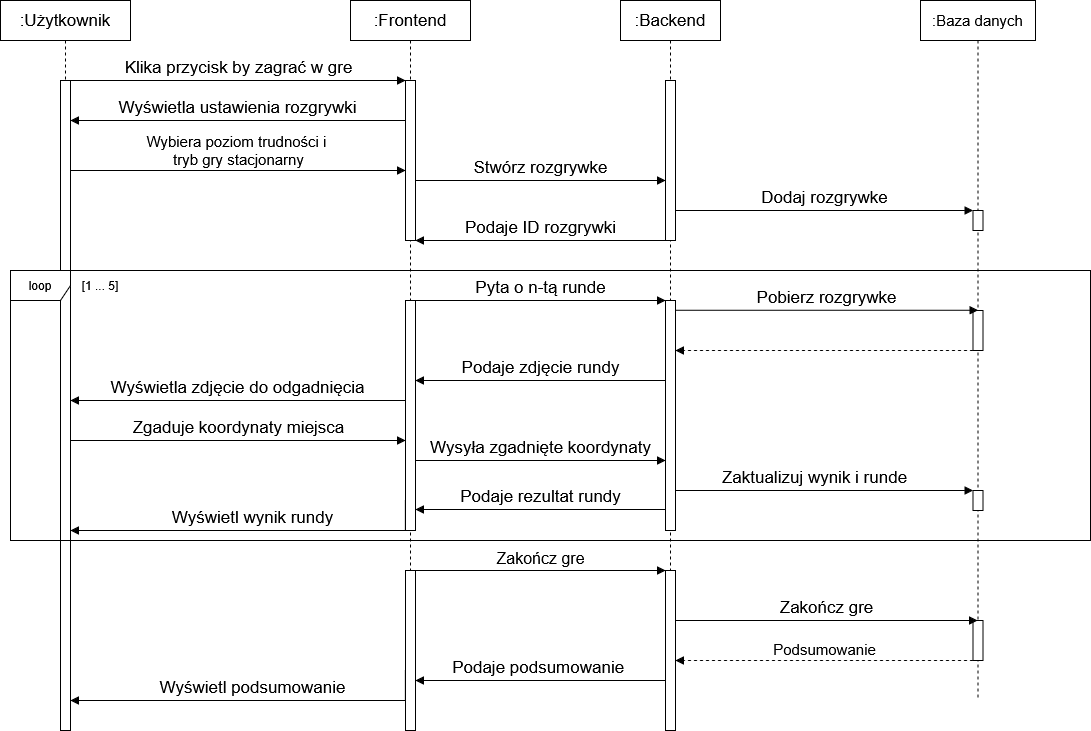
\includegraphics[width=1.2\textwidth]{./images/standardGameplaySequenceDiagram.png}}
    \caption{Diagram sekwencji przedstawiający przebieg rozgrywki w aplikacji UniGuesser}
    \label{fig:sequence-diagram}
\end{figure}

\section{Estetyka i design (Filip Jezierski) }
Wygląd aplikacji został zaprojektowany z myślą o prostocie, intuicyjności oraz atrakcyjności wizualnej. Poniżej przedstawiono kluczowe elementy designu interfejsu użytkownika.

\subsection{Ogólny projekt interfejsu}
Design interfejsu użytkownika naszej aplikacji skupia się na minimalizmie i czytelności. Stosowane są przyjęte jako standardowe układy elementów, takie jak menu nawigacji w górnej części ekranu, co ułatwia poruszanie się po aplikacji, nawet dla nowych użytkowników. Podstrony są zaprojektowane tak, aby unikać nadmiaru informacji, co pozwala użytkownikom skupić się na kluczowych funkcjonalnościach. W trakcie rozgrywki centralnym elementem interfejsu jest interaktywna mapa, która umożliwia użytkownikom łatwe wskazywanie lokalizacji, a pozostałe elementy interfejsu są rozmieszczone w sposób intuicyjny wokół niej.

\subsection{Kolorystyka}
% todo: screen z aplikacji
Aplikacja wykorzystuje dwukolorową paletę barw, opartą na odcieniach białego i ciemnoniebieskiego, inspirowaną kolorystyką Politechniki Gdańskiej. Biały kolor dominuje w tle, co zapewnia czystość i przejrzystość interfejsu, natomiast niebieskie akcenty są używane do wyróżnienia kluczowych elementów, takich jak przyciski, nagłówki czy linki. Przykładowe zastosowanie palety kolorów przedstawia rysunek \ref{fig:register-form}. Taka kolorystyka zapewnia odpowiedni kontrast i ułatwia czytelność tekstu, zwłaszcza przy korzystaniu z aplikacji w różnych warunkach oświetleniowych, co jest szczególnie istotne ze względu na terenowy charakter gry.

\begin{figure}[H]
    \centering
    \makebox[\textwidth]{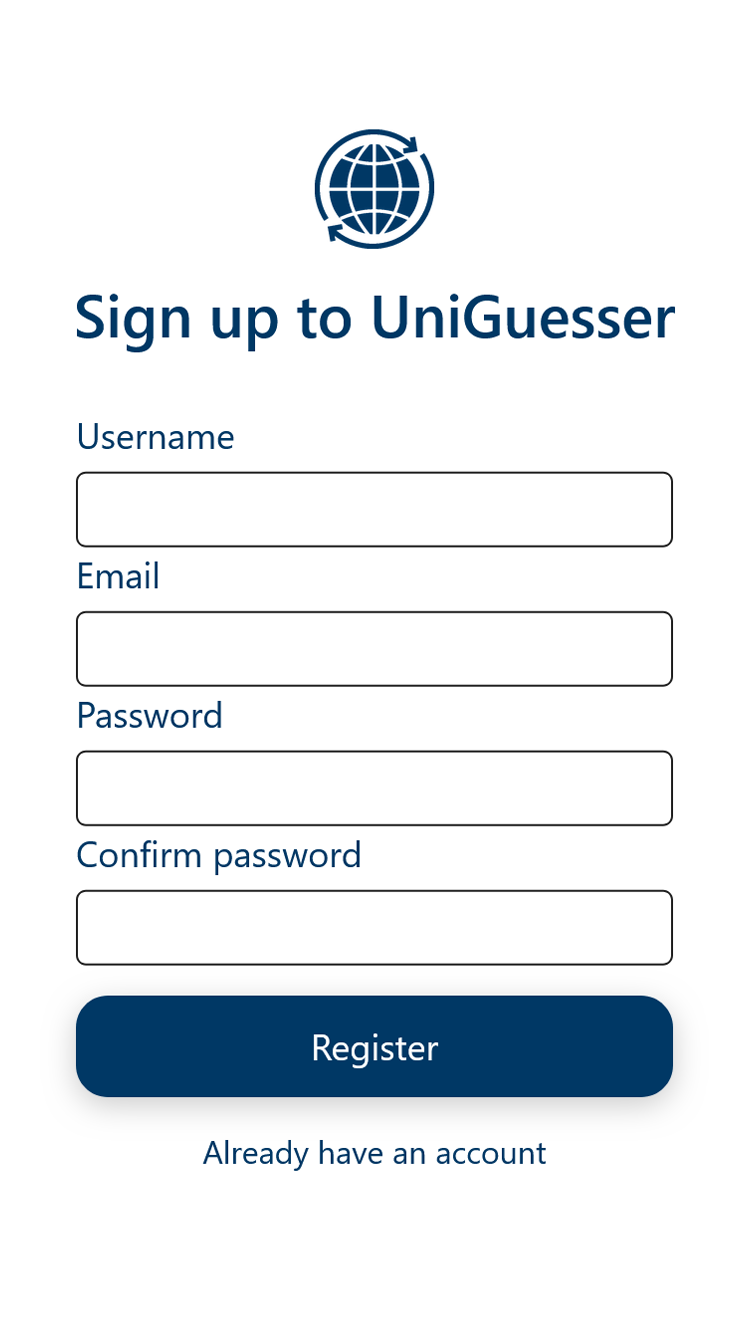
\includegraphics[width=0.5\textwidth]{./images/registerForm.png}}
    \caption{Przykładowy ekran rejestracji użytkownika w aplikacji UniGuesser, ilustrujący zastosowaną kolorystykę}
    \label{fig:register-form}
\end{figure}

\subsection{Typografia}
Aplikacja wykorzystuje czcionkę Roboto, która jest nowoczesna, czytelna i estetyczna. Czcionka ta jest szeroko stosowana w projektach webowych ze względu na swoją uniwersalność i dobrą czytelność na ekranach o różnych rozdzielczościach.

\subsection{Ikony}
W interfejsie użytkownika wykorzystano zestaw prostych i intuicyjnych ikon, pochodzących z biblioteki Google Icons. Ikony te są spójne stylistycznie i pomagają użytkownikom szybko zidentyfikować funkcje oraz akcje dostępne w aplikacji. Dzięki zastosowaniu powszechnie rozpoznawalnych symboli, nawigacja staje się bardziej intuicyjna, co przekłada się na lepsze doświadczenie użytkownika.

\subsection{Responsywność}
Aplikacja została zaprojektowana z myślą o responsywności, co oznacza, że dostosowuje się do różnych rozmiarów ekranów i urządzeń. Dzięki temu użytkownicy mogą korzystać z aplikacji zarówno na komputerach stacjonarnych, jak i urządzeniach mobilnych, bez utraty funkcjonalności czy estetyki. Elementy interfejsu, takie jak przyciski, formularze czy mapy, automatycznie dostosowują swoje rozmiary i układ w zależności od dostępnej przestrzeni ekranowej. Na mniejszych ekranach, takich jak smartfony, menu nawigacyjne jest ukryte za ikoną hamburgera, co pozwala zaoszczędzić miejsce i utrzymać przejrzystość interfejsu. Ponadto, kluczowe funkcje pozostają łatwo dostępne, a tekst i grafiki są skalowane odpowiednio do rozdzielczości ekranu, zapewniając optymalne doświadczenie użytkownika niezależnie od urządzenia.

\chapter{Projekt systemu (Michał Turski i Filip Jezierski)}
\label{chap:system_project}
Niniejszy rozdział przedstawia szczegółowy projekt systemu aplikacji webowej \textbf{UniGuesser}. Opisane zostaną kluczowe elementy architektury systemu, w tym warstwy aplikacji, baza danych oraz najbardziej kluczowe interakcje użytkownika z systemem. Zaczynając od ogólnego przeglądu architektury, przejdziemy do szczegółowego omówienia poszczególnych komponentów i ich wzajemnych relacji.

W aplikacji zastosowano architekturę warstwową, której szczegółowa implementacja zostanie opisana w niniejszym rozdziale. Na najwyższym poziomie abstrakcji system można podzielić na trzy główne warstwy: warstwę prezentacji (frontend), warstwę logiki biznesowej (backend) oraz warstwę persystencji danych (baza danych). Podział ten odzwierciedla sposób izolowania odpowiedzialności poszczególnych komponentów. Dzięki temu użytkownik komunikuje się z aplikacją poprzez interfejs użytkownika, który następnie przekazuje żądania do warstwy logiki biznesowej. Ta z kolei przetwarza żądania, wykonuje odpowiednie operacje i komunikuje się z bazą danych w celu przechowywania lub pobierania danych.

\begin{figure}[h]
    \centering
    
\includegraphics[width=1.0\textwidth]{./images/architecture-overview.png}
    \caption{Uproszczony schemat architektury systemu UniGuesser – ogólny podział na warstwy}
    \label{fig:architecture-overview}
\end{figure}


\section{Architektura logiki biznesowej (Michał Turski)}
Architektura w aplikacji \textbf{UniGuesser} została zbudowana w oparciu o Command-Query Responsibility Segregation (CQRS) oraz Domain-Driven Design (DDD), które
są obecnie standardem w wytwarzaniu oprogramowania. [dodać źródło na potwierdznie słów]
Ponadto zdecydowaliśmy na wybór architektury monolitycznej ze względu na szybkość rozwoju i łatwość wdrożenia, co pomogło skupić się nam na aspekcie funkcjonalnym aplikacji w początkowej fazie jej tworzenia.

\subsection{Wzorzec CQRS (Command Query Responsibility Segregation)}
Wykorzystany został również wzorzec CQRS. Zakłada on rozdzielenie operacji modyfikujących stan systemu (komendy) od operacji, które odczytują dane (zapytania). Pozwala to na lepsze skalowanie i rozdzielenie logiki aplikacji. Dzięki temu można optymalizować każdą z tych operacji niezależnie, co przekłada się na wydajność i czytelność kodu. W kontekście skalowalności systemu zastosowano uproszczoną implementację wzorca CQRS z pojedynczą bazą danych, która jest wystarczająca przy przewidywanym obciążeniu nieprzekraczającym 50 zapytań na sekundę. Taka architektura zapewnia odpowiednią wydajność przy jednoczesnym zachowaniu prostoty infrastruktury.

\begin{figure}[h]
    \centering
    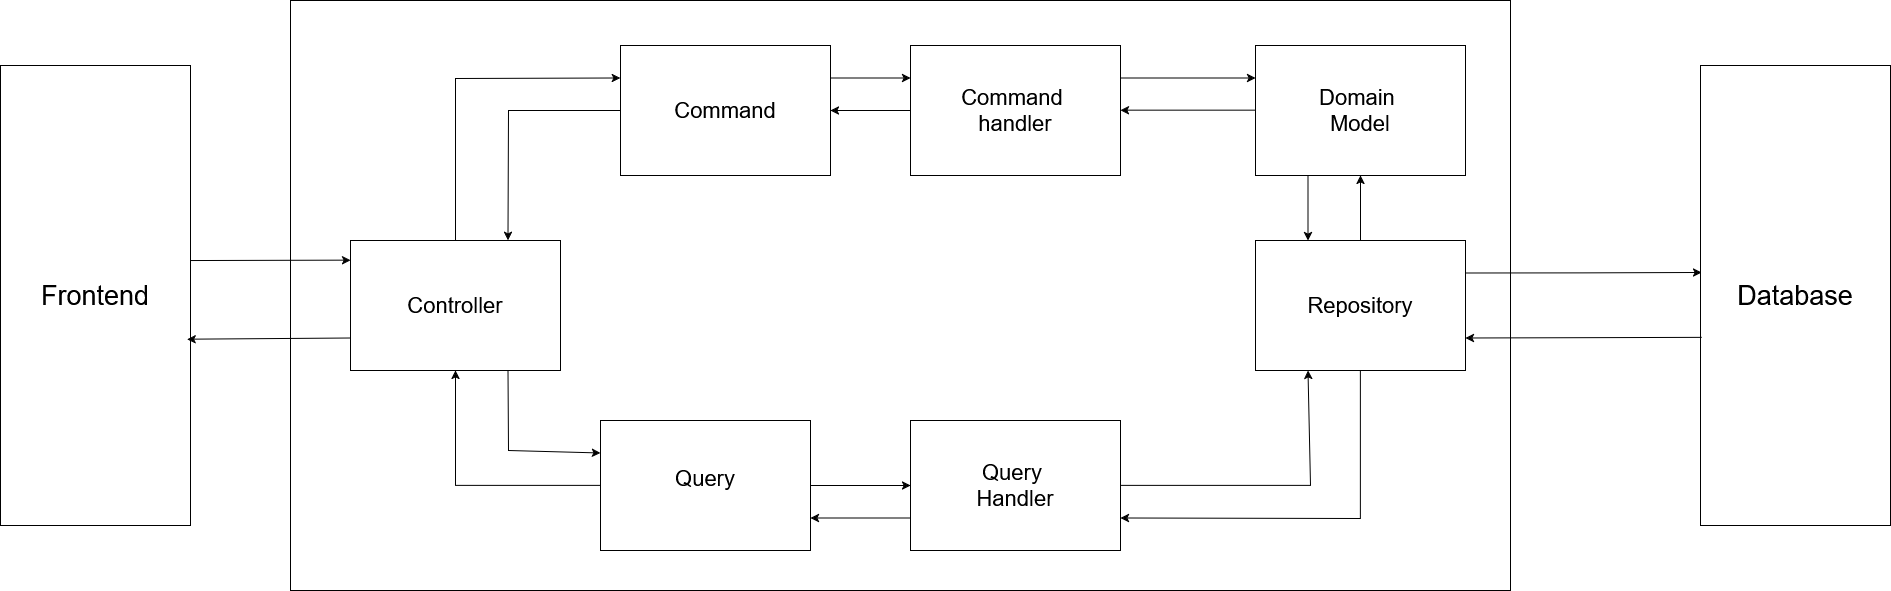
\includegraphics[width=1.0\textwidth]{./images/cqrs-communication.png}
    \caption{Schemat komunikacji przy zastosowaniu wzorca CQRS}
    \label{fig:cqrs-communication}
\end{figure}



\subsection{Zastosowanie DDD (Domain-Driven Design)}
Model systemu został zaprojektowany zgodnie z podejściem Domain-Driven Design (DDD), które kładzie nacisk na zrozumienie i modelowanie domeny problemowej. W aplikacji definiujemy trzy główne warstwy DDD: warstwę domeny, warstwę aplikacji oraz warstwę infrastruktury. Każda z warstw znajduje się w osobnym module, co ułatwia zarządzanie kodem i jego rozwój. Dodatkowo w aplikacji wydzielony został czwarty moduł „API”, który odpowiada za komunikację z warstwą prezentacji, co zmniejsza złożoność warstwy aplikacji. Moduł „API” obsługuje zarówno zapytania, jak i komendy, delegując je odpowiednio do warstwy aplikacji, która następnie komunikuje się z warstwą domeny i infrastruktury w celu realizacji żądanych operacji.

\section{Baza danych (Michał Turski)}

W aplikacji zastosowano relacyjną bazę danych, do przechowywania informacji o aktualnych i przeszłych sesjach gier, użytkownikach, lokalizacjach oraz wynikach. Zdecydowaliśmy się na wykorzystanie relacyjnej bazy danych ze względu na duża ilość powiąza między encjami oraz potrzebę zapewnienia integralności danych między nimi. Relacyjne bazy danych zapewniaja ACID (Atomicity, Consistency, Isolation, Durability), co jest kluczowe dla zachowania spójności danych w rozgrywce. 

\subsection{Diagram ERD}
Przedstawiony na rysunku \ref{fig:erd-diagram} diagram ERD (Entity-Relationship Diagram) ilustruje strukturę bazy danych aplikacji UniGuesser, pokazując główne tabele oraz relacje między nimi. Użytkownik może posiadać wiele sesji gier, a każda sesja ma określoną liczbę rund, z których każda posiada przypisaną do siebie lokacje. Ponadto każde miejsce może mieć swojego autora (użytkownika), który dodał je do bazy danych. 

\begin{figure}[h]
    \centering
    
\includegraphics[width=1.0\textwidth]{./images/erdDiagram.png}
    \caption{Diagram ERD (Entity-Relationship Diagram) dla bazy danych aplikacji UniGuesser}
    \label{fig:erd-diagram}
\end{figure}

\subsection{Opis głównych tabel i związków}

\begin{itemize}
    \item \textbf{Users (Użytkownicy)} – tabela przechowująca informacje o użytkownikach aplikacji.
\end{itemize}

\begin{table}[H]
\centering
\renewcommand{\arraystretch}{1.2}
\begin{tabular}{|p{2.5cm}|p{8cm}|p{2.5cm}|}
\hline
\textbf{Atrybut} & \textbf{Opis} & \textbf{Typ / Uwagi} \\ \hline
ID & Unikalny identyfikator użytkownika. & Klucz główny \\ \hline
Nickname & Unikalna nazwa użytkownika. & Tekst \\ \hline
Email & Unikalny adres e-mail użytkownika. & Tekst \\ \hline
PasswordHash & Zaszyfrowane hasło użytkownika. & Tekst \\ \hline
CreatedAt & Data i czas utworzenia konta. & Data/Czas \\ \hline
Role & Rola użytkownika w systemie (np. użytkownik, administrator). & Enumeracja \\ \hline
\end{tabular}
\caption{Tabela \texttt{Users}}
\end{table}

\textbf{GameSessions (Sesje gier)} – tabela przechowująca informacje o aktywnych i zakończonych rozgrywkach.

\begin{table}[H]
\centering
\renewcommand{\arraystretch}{1.2}
\begin{tabular}{|p{2.8cm}|p{8.5cm}|p{2cm}|}
\hline
\textbf{Atrybut} & \textbf{Opis} & \textbf{Typ / Uwagi} \\ \hline
ID & Unikalny identyfikator sesji gry. & Klucz główny \\ \hline
GameMode & Tryb gry w danej sesji. & Enumeracja \\ \hline
GameEndDate & Data, do której rozgrywka jest aktywna. & Data/Czas \\ \hline
RoundNumber & Aktualnie rozgrywana runda. & Liczba \\ \hline
GameScore & Łączna liczba punktów zdobytych. & Liczba całkowita \\ \hline
Difficulty & Poziom trudności sesji. & Enumeracja \\ \hline
FinishedTime & Data zakończenia rozgrywki. & Data/Czas \\ \hline
UserID & Identyfikator użytkownika. & Klucz obcy → Users \\ \hline
\end{tabular}
\caption{Tabela \texttt{GameSessions}}
\end{table}

\textbf{Rounds (Rundy)} – tabela przechowująca informacje o poszczególnych rundach w sesji gry.

\begin{table}[H]
\centering
\renewcommand{\arraystretch}{1.2}
\begin{tabular}{|p{3cm}|p{8.5cm}|p{1.8cm}|}
\hline
\textbf{Atrybut} & \textbf{Opis} & \textbf{Typ / Uwagi} \\ \hline
ID & Unikalny identyfikator rundy. & Klucz główny \\ \hline
GuessedLatitude & Szerokość geograficzna wskazana przez użytkownika. & Liczba zmiennoprzecinkowa \\ \hline
GuessedLongitude & Długość geograficzna wskazana przez użytkownika. & Liczba zmiennoprzecinkowa \\ \hline
Score & Punkty zdobyte w rundzie. & Liczba całkowita \\ \hline
GameSessionID & Identyfikator sesji gry. & Klucz obcy → GameSessions \\ \hline
LocationID & Identyfikator lokacji. & Klucz obcy → Places \\ \hline
\end{tabular}
\caption{Tabela \texttt{Rounds}}
\end{table}

\textbf{Places (Lokacje)} – tabela przechowująca informacje o lokacjach dostępnych w grze.

\begin{table}[H]
\centering
\renewcommand{\arraystretch}{1.2}
\begin{tabular}{|p{2.5cm}|p{8cm}|p{2.5cm}|}
\hline
\textbf{Atrybut} & \textbf{Opis} & \textbf{Typ / Uwagi} \\ \hline
ID & Unikalny identyfikator lokacji. & Klucz główny \\ \hline
Name & Nazwa lokacji. & Tekst \\ \hline
Description & Opis lokacji. & Tekst \\ \hline
Latitude & Szerokość geograficzna lokacji. & Liczba zmiennoprzecinkowa \\ \hline
Longitude & Długość geograficzna lokacji. & Liczba zmiennoprzecinkowa \\ \hline
Difficulty & Poziom trudności lokacji. & Enumeracja \\ \hline
ImageUrl & Adres URL obrazu lokacji. & Tekst \\ \hline
AltImage & Tekst alternatywny dla obrazu lokacji. & Tekst \\ \hline
CreationTime & Data i czas dodania lokacji. & Data/Czas \\ \hline
AuthorID & Identyfikator autora lokacji. & Klucz obcy → Users \\ \hline
\end{tabular}
\caption{Tabela \texttt{Places}}
\end{table}

\section{Analiza interakcji użytkownika z systemem (Michał Turski)}
W rozdziale przedstawione zostaną możliwości i przebieg kluczowych funkcjonalności aplikacji UniGuesser z perspektywy użytkownika końcowego. Opisane zostaną główne przypadki użycia oraz interakcje między użytkownikiem a systemem podczas typowej rozgrywki.

\subsection{Przypadki użycia aplikacji}
Przedstawiony na rysunku \ref{fig:use-case-diagram} diagram przypadków użycia ilustruje główne funkcjonalności aplikacji UniGuesser z perspektywy użytkownika moderatora i administratora. Użytkownik może rejestrować się i logować do systemu, rozpoczynać nowe sesje gier, uczestniczyć w rozgrywkach, przeglądać wyniki innych użytkowników, oraz proponować nowe lokacje. Moderator dodatkowo może zatwierdzać lub odrzucać proponowane lokacje, natomiast administrator ma uprawnienia do zarządzania użytkownikami.

\begin{figure}[H]
    \centering
    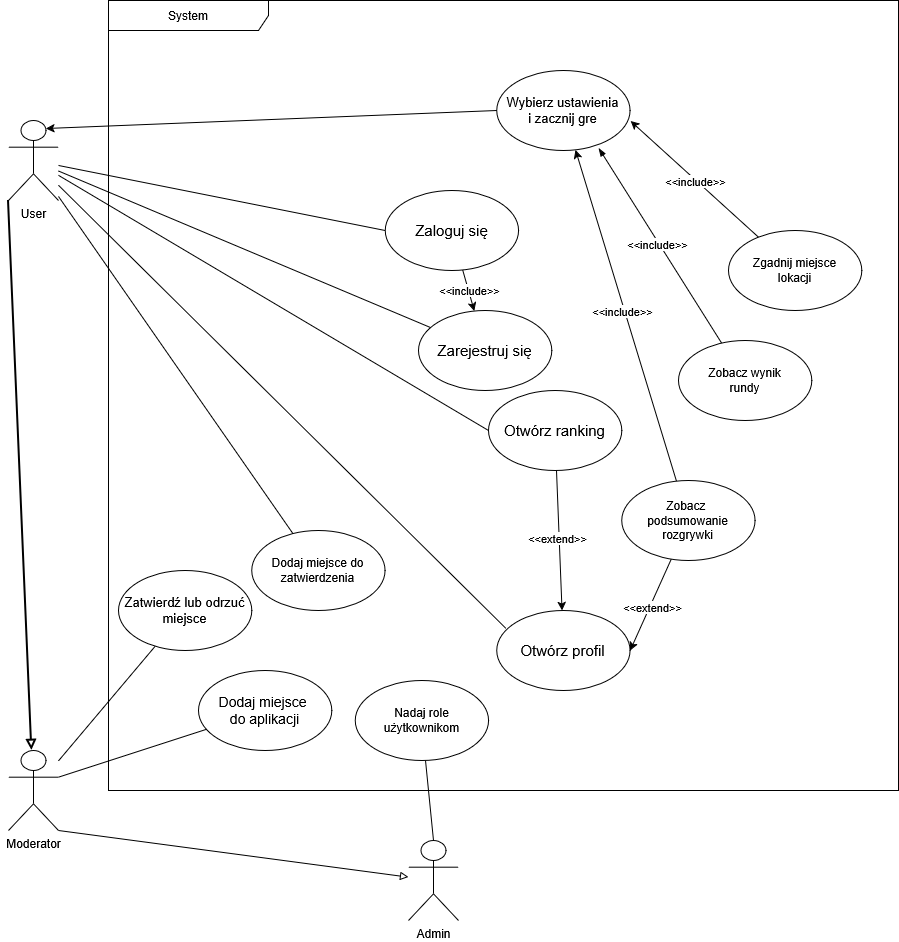
\includegraphics[width=1.0\textwidth]{./images/useCaseDiagram.png}
    \caption{Diagram przypadków użycia aplikacji UniGuesser}
    \label{fig:use-case-diagram}
\end{figure}

\subsection{Diagram sekwencji rozgrywki}

Diagram sekwencji przedstawiony na rysunku \ref{fig:sequence-diagram} ilustruje przebieg interakcji między użytkownikiem a systemem podczas typowej rozgrywki w aplikacji UniGuesser. Proces rozpoczyna się od momentu, gdy użytkownik uruchamia nową grę, poprzez kolejne rundy, aż do momentu zakończenia sesji i wyświetlenia wyników końcowych.

\begin{figure}[H]
    \centering
    \makebox[\textwidth]{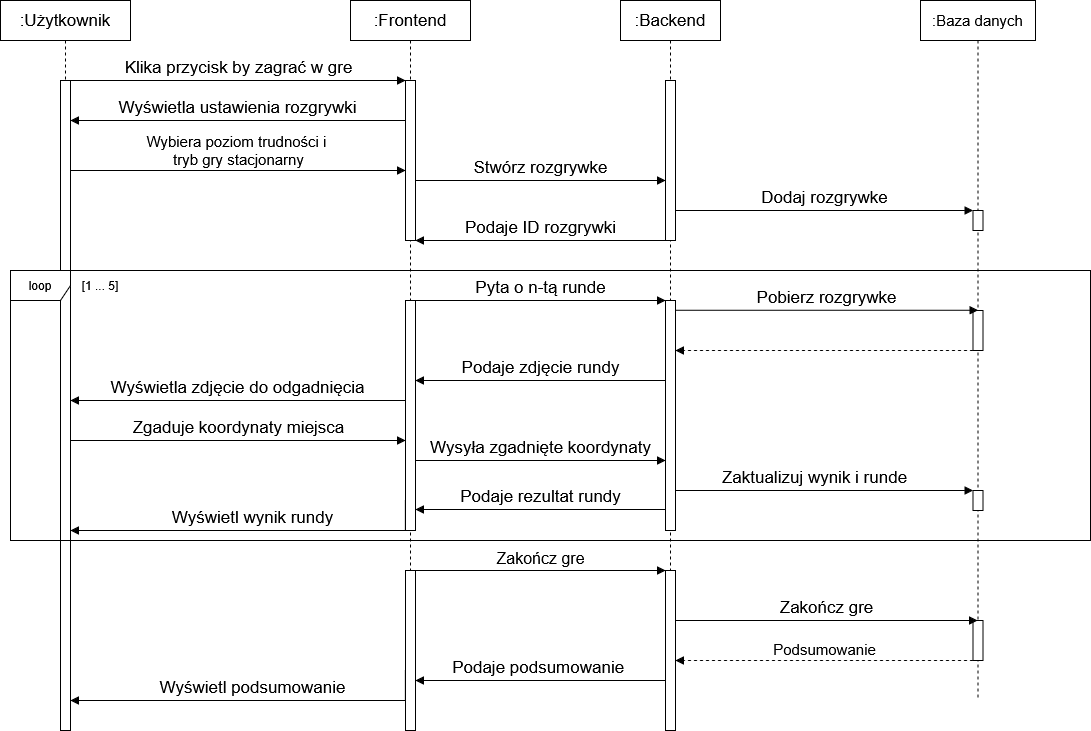
\includegraphics[width=1.2\textwidth]{./images/standardGameplaySequenceDiagram.png}}
    \caption{Diagram sekwencji przedstawiający przebieg rozgrywki w aplikacji UniGuesser}
    \label{fig:sequence-diagram}
\end{figure}

\section{Estetyka i design (Filip Jezierski) }
Wygląd aplikacji został zaprojektowany z myślą o prostocie, intuicyjności oraz atrakcyjności wizualnej. Poniżej przedstawiono kluczowe elementy designu interfejsu użytkownika.

\subsection{Ogólny projekt interfejsu}
Design interfejsu użytkownika naszej aplikacji skupia się na minimalizmie i czytelności. Stosowane są przyjęte jako standardowe układy elementów, takie jak menu nawigacji w górnej części ekranu, co ułatwia poruszanie się po aplikacji, nawet dla nowych użytkowników. Podstrony są zaprojektowane tak, aby unikać nadmiaru informacji, co pozwala użytkownikom skupić się na kluczowych funkcjonalnościach. W trakcie rozgrywki centralnym elementem interfejsu jest interaktywna mapa, która umożliwia użytkownikom łatwe wskazywanie lokalizacji, a pozostałe elementy interfejsu są rozmieszczone w sposób intuicyjny wokół niej.

\subsection{Kolorystyka}
% todo: screen z aplikacji
Aplikacja wykorzystuje dwukolorową paletę barw, opartą na odcieniach białego i ciemnoniebieskiego, inspirowaną kolorystyką Politechniki Gdańskiej. Biały kolor dominuje w tle, co zapewnia czystość i przejrzystość interfejsu, natomiast niebieskie akcenty są używane do wyróżnienia kluczowych elementów, takich jak przyciski, nagłówki czy linki. Przykładowe zastosowanie palety kolorów przedstawia rysunek \ref{fig:register-form}. Taka kolorystyka zapewnia odpowiedni kontrast i ułatwia czytelność tekstu, zwłaszcza przy korzystaniu z aplikacji w różnych warunkach oświetleniowych, co jest szczególnie istotne ze względu na terenowy charakter gry.

\begin{figure}[H]
    \centering
    \makebox[\textwidth]{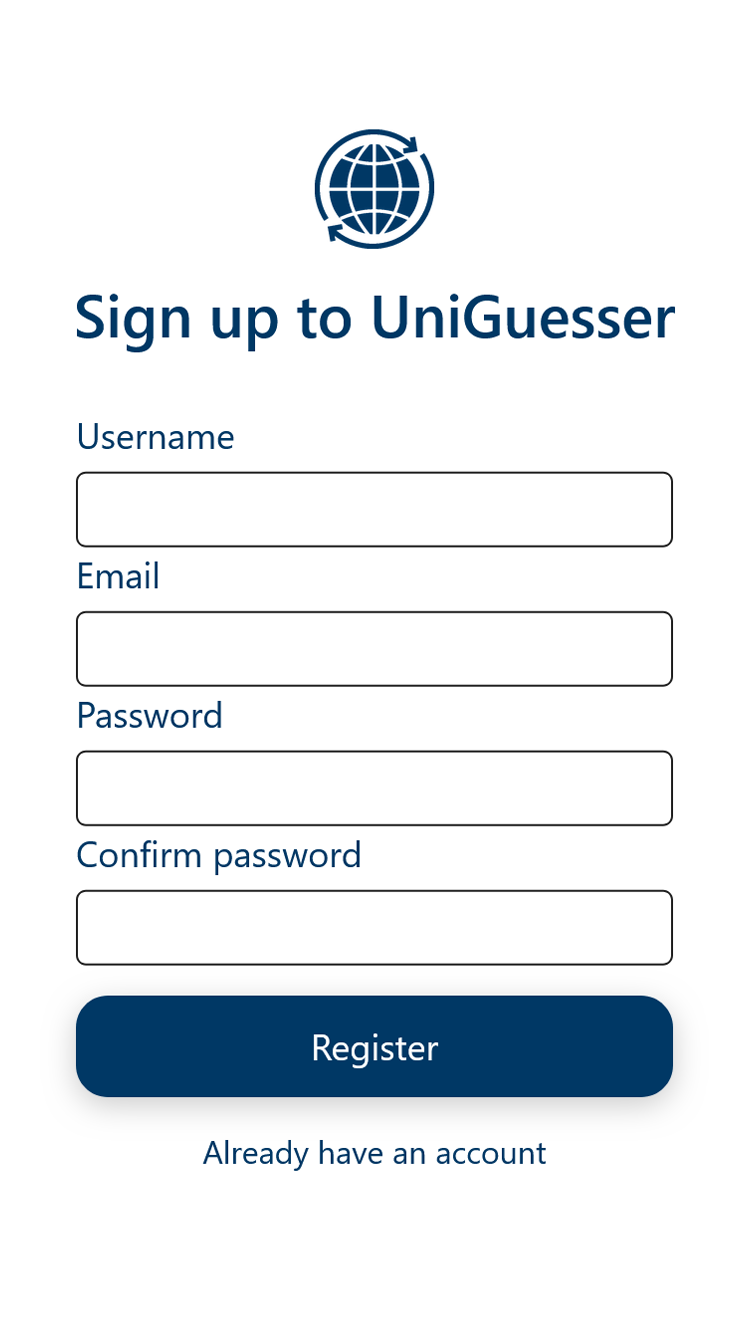
\includegraphics[width=0.5\textwidth]{./images/registerForm.png}}
    \caption{Przykładowy ekran rejestracji użytkownika w aplikacji UniGuesser, ilustrujący zastosowaną kolorystykę}
    \label{fig:register-form}
\end{figure}

\subsection{Typografia}
Aplikacja wykorzystuje czcionkę Roboto, która jest nowoczesna, czytelna i estetyczna. Czcionka ta jest szeroko stosowana w projektach webowych ze względu na swoją uniwersalność i dobrą czytelność na ekranach o różnych rozdzielczościach.

\subsection{Ikony}
W interfejsie użytkownika wykorzystano zestaw prostych i intuicyjnych ikon, pochodzących z biblioteki Google Icons. Ikony te są spójne stylistycznie i pomagają użytkownikom szybko zidentyfikować funkcje oraz akcje dostępne w aplikacji. Dzięki zastosowaniu powszechnie rozpoznawalnych symboli, nawigacja staje się bardziej intuicyjna, co przekłada się na lepsze doświadczenie użytkownika.

\subsection{Responsywność}
Aplikacja została zaprojektowana z myślą o responsywności, co oznacza, że dostosowuje się do różnych rozmiarów ekranów i urządzeń. Dzięki temu użytkownicy mogą korzystać z aplikacji zarówno na komputerach stacjonarnych, jak i urządzeniach mobilnych, bez utraty funkcjonalności czy estetyki. Elementy interfejsu, takie jak przyciski, formularze czy mapy, automatycznie dostosowują swoje rozmiary i układ w zależności od dostępnej przestrzeni ekranowej. Na mniejszych ekranach, takich jak smartfony, menu nawigacyjne jest ukryte za ikoną hamburgera, co pozwala zaoszczędzić miejsce i utrzymać przejrzystość interfejsu. Ponadto, kluczowe funkcje pozostają łatwo dostępne, a tekst i grafiki są skalowane odpowiednio do rozdzielczości ekranu, zapewniając optymalne doświadczenie użytkownika niezależnie od urządzenia.

\chapter{Implementacja}
\label{chap:implementation}
\section{Implementacja wyglądu i funkcjonalności frontendu}
W tej sekcji omówione zostaną kluczowe aspekty implementacji frontendu aplikacji, w tym architektura, struktura UI i komponentów, warstwa wizualna, obsługa interakcji użytkownika, integracja z geolokalizacją, implementacja trybów gry, komunikacja z backendem oraz mechanizmy PWA.

\subsection{Architektura frontendu (Karina Wołoszyn)}

\subsection{Struktura UI i komponentów (Karina Wołoszyn)}

\subsection{Warstwa wizualna (Karina Wołoszyn)}

\subsection{Obsługa interakcji użytkownika (Karina Wołoszyn)}

\subsection{Integracja z geolokalizacją (Filip Jezierski)}

\subsection{Implementacja trybów gry (Filip Jezierski)}

\subsection{Komunikacja z backendem (Filip Jezierski)}

\subsection{Mechanizmy PWA (Filip Jezierski)}

% \subsection{Problemy napotkane  przy implementacji frontendu}


\section{Implementacja backendu i logiki aplikacji}

W tej sekcji omówione zostaną kluczowe aspekty implementacji backendu aplikacji, rozgrywki  mechanizmy autoryzacji i uwierzytelniania użytkowników, zarządzanie danymi oraz obsługa błędów, a także problemy, które napotkano podczas implementacji.

\subsection{Implementacja rozgrywki}

Przedstawienie sposobu w jaki została zaimplementowana rozgrywka z \ref{fig:sequence-diagram} w aplikacji. 

Proces rozpoczęcia rozgrywki inicjuje wywołanie kontrolera \texttt{api/game/start}, który odpowiada za utworzenie nowej \textit{Sesji Rozgrywki} (\ref{tab:game-sessions}).
W ramach tego etapu backend generuje odpowiednią liczbę rund (\ref), przypisuje im losowe miejsca do zgadnięcia, nadaje sesji status \texttt{InProgress}, a następnie zwraca unikalny identyfikator gry w postaci GUID.
W przypadku użytkownika niezalogowanego aplikacja dodatkowo generuje i zwraca tymczasowy token, który umożliwia jego uwierzytelnienie w kolejnych żądaniach.

Aby pobrać dane dotyczące danej rundy, frontend wywołuje endpoint
\texttt{api/game/{gameId}/round/{roundNumber}},
gdzie \texttt{gameId} jest identyfikatorem sesji, a \texttt{roundNumber} – numerem aktualnej rundy. Backend zwraca ścieżkę do obrazu przedstawiającego miejsce, które należy odgadnąć. Obraz może być przechowywany lokalnie na serwerze lub stanowić odnośnik do zewnętrznego źródła.


Odpowiedź użytkownika jest obsługiwana przez endpoint
\texttt{api/game/{gameId}/round/{roundNumber}/check}.
Aplikacja weryfikuje lokalizację podaną przez użytkownika, oblicza odległość pomiędzy faktycznym miejscem a wskazanym punktem oraz na tej podstawie przyznaje punkty za daną rundę.

Po zakończeniu wszystkich rund gracz wywołuje endpoint
\texttt{api/game/{gameId}/finish},
który finalizuje rozgrywkę. Backend podsumowuje wyniki, aktualizuje status sesji na \texttt{Completed} i zwraca końcowy rezultat użytkownikowi.
Dla użytkowników zalogowanych rezultat jest trwale zapisywany w bazie, natomiast dla użytkowników niezalogowanych sesja jest automatycznie usuwana po upływie jednej godziny.


\subsection{Autoryzacja i uwierzytelnianie użytkowników}


\textbf{Generowanie i struktura tokenu JWT służącego do autoryzacji użytkowników}

W celu autoryzacji wykorzystany został JSON Web Token. Jest to standard wymiany informacji między dwoma stronami w formie obiektu JSON, który jest bezpiecznie podpisany cyfrowo. 

Składa się on z trzech niezależnych części zakodowanych w formacie Base64: nagłówka (header), ładunku (payload) oraz podpisu (signature). Nagłówek zawiera informacje o algorytmie podpisu i typie tokenu, ładunek zawiera dane użytkownika i inne informacje, a podpis służy do weryfikacji integralności tokenu i autentyczności nadawcy.

Przykładowy token JWT:
\begin{lstlisting}
eyJhbGciOiJIUzI1NiIsInR5cCI6IkpXVCJ9.eyJzdWIiOiIxMjM0NTY3ODkwIiwibmFtZSI
6IkpvaG4gRG9lIiwiYWRtaW4iOnRydWUsImlhdCI6MTUxNjIzOTAyMn0.KMUFsIDTnFmyG3n
MiGM6H9FNFUROf3wh7SmqJp-QV30
\end{lstlisting}

Nagłówek przedstawia zakodowane informacje o algorytmie podpisu oraz typie tokenu (w tym przypadku HS256):

\begin{lstlisting}
{
  "alg": "HS256",
  "typ": "JWT"
}
\end{lstlisting}

Payload zawiera zakodowane informacje, które chcemy przekazać, jak np. identyfikator użytkownika, nazwa użytkownika, role itp.:

\begin{lstlisting}
{
  "ID": "23141",
  "name": "Jan Kowalski",
  "admin": true,
  "iat": 1516239022
}
\end{lstlisting}

Podpis jest generowany przez zakodowanie nagłówka i payloadu oraz podpisanie ich kluczem prywatnym przy użyciu algorytmu określonego w nagłówku.

W środowisku .NET mechanizm tokenów JWT jest wspierany przez bibliotekę \texttt{Microsoft.AspNetCore.Authentication.JwtBearer}, która umożliwia łatwą integrację z mechanizmami uwierzytelniania i autoryzacji w aplikacjach ASP.NET Core. Dzięki temu jesteśmy w stanie generować w efektywny sposób tokeny, które wykorzystywane są do autoryzacji. 

\begin{lstlisting}[language={[Sharp]C}, caption={Generowanie tokenu JWT w warstwie backendu}, label={lst:jwt-generation}]
var claims = new List<Claim>
{
    new(ClaimTypes.NameIdentifier, user.Id.ToString()),
    new(ClaimTypes.Email, user.Email),
    new(ClaimTypes.Role, user.Role),
    new(ClaimTypes.Name, user.Nickname),
    new("token_type", "user")
};

// Klucz podpisujący token (HMAC SHA-256)
var key = new SymmetricSecurityKey(
    Encoding.UTF8.GetBytes(_authenticationSettings.JwtKey));

// Poświadczenia podpisu
var credentials = new SigningCredentials(
    key, SecurityAlgorithms.HmacSha256);

// Czas wygaśnięcia tokenu
var expires = DateTime.Now.AddMinutes(
    _authenticationSettings.JwtExpireAccount);

// Utworzenie obiektu tokenu JWT
var token = new JwtSecurityToken(
    issuer: _authenticationSettings.JwtIssuer,
    audience: _authenticationSettings.JwtIssuer,
    claims: claims,
    expires: expires,
    signingCredentials: credentials
);
\end{lstlisting}

\textbf{Identyfikowanie użytkowników i autoryzacja dostępu do zasobów}

W aplikacji wykorzystano mechanizm autoryzacji oparty na atrybutach \texttt{[Authorize]} dostępnych w ASP.NET Core. Atrybut ten pozwala na zabezpieczenie kontrolerów lub konkretnych akcji, wymagając od użytkownika posiadania ważnego tokenu JWT oraz odpowiednich uprawnień (ról) do dostępu do zasobów. 
Na etapie przetwarzania żądania, middleware uwierzytelniające sprawdza obecność i ważność tokenu JWT w nagłówku autoryzacji. Jeśli token jest poprawny, użytkownik zostaje zidentyfikowany, a jego rola jest sprawdzana w kontekście żądanej akcji.


\textbf{Hashowanie haseł użytkowników i uwierzytelnianie}

Do bezpiecznego generowania i przechowywania haseł użytkowników wykorzystano .NET Core Identity, który implementuje algorytm HMAC-SHA256. Algorytm ten jest odporny na ataki brute-force dzięki zastosowaniu kosztownego obliczeniowo procesu hashowania oraz losowego saltingu. W procesie rejestracji hasło użytkownika jest hashowane przed zapisem do bazy danych, natomiast podczas logowania następuje weryfikacja hasła poprzez porównanie jego hasha z wartością przechowywaną w bazie.

\begin{lstlisting}[language={[Sharp]C}, caption={Hashowanie i weryfikacja hasła użytkownika}]
// Hashowanie hasła podczas rejestracji
var passwordHash = passwordHasher.HashPassword(
    newUser, 
    registerAccountCommand.Password
);

// Weryfikacja hasła podczas logowania
var result = passwordHasher.VerifyHashedPassword(
    user, 
    user.PasswordHash, 
    loginCommand.Password
);
\end{lstlisting}

\subsection{Walidacja danych}
    W celu zapewnienia poprawności danych wejściowych w aplikacji zastosowano bibliotekę FluentValidation. Umożliwia ona definiowanie reguł walidacyjnych w sposób deklaratywny, czytelny i łatwy w utrzymaniu. Przykładowo, podczas rejestracji użytkownika można zdefiniować reguły dotyczące minimalnej i maksymalnej długości hasła, prawidłowego formatu adresu e-mail oraz unikalności nazwy użytkownika w systemie. Dzięki temu możliwe jest centralne zarządzanie walidacją oraz zapewnienie spójności danych w całej aplikacji. 
    
    Biblioteka FluentValidation jest w pełni zintegrowana z mechanizmem wiązania modeli (model binding) w ASP.NET Core, co umożliwia automatyczne wywoływanie walidacji podczas przetwarzania żądań HTTP. W przypadku wykrycia błędów walidacji framework automatycznie zwraca odpowiedź HTTP 400 (Bad Request) wraz ze szczegółowym opisem napotkanych problemów, co znacząco ułatwia debugowanie i poprawia komunikację z klientem API.

    Niektóre reguły walidacyjne wymagają dostępu do warstwy persystencji, na przykład w celu sprawdzenia, czy w bazie danych nie istnieje już użytkownik o podanym adresie e-mail lub nazwie. W takich przypadkach do konstruktora klasy walidatora wstrzykiwane są odpowiednie repozytoria poprzez mechanizm wstrzykiwania zależności (Dependency Injection). 

\begin{lstlisting}[language={[Sharp]C}, caption={Przykład walidacji danych użytkownika podczas rejestracji}, label={lst:fluent-validation}]
public class RegisterUserDtoValidator : AbstractValidator<RegisterUserDto>
{
    private readonly IAccountRepository _accountRepository;

    public RegisterUserDtoValidator(IAccountRepository accountRepository)
    {
        _accountRepository = accountRepository;
        RuleFor(u => u.Email)
            .NotEmpty()
            .EmailAddress();

        RuleFor(u => u.Nickname)
            .NotEmpty()
            .MinimumLength(3)
            .MaximumLength(25);

        RuleFor(u => u.Password)
            .NotEmpty()
            .MinimumLength(8)
            .WithMessage("Minimum length of password is 8");

        RuleFor(x => x.ConfirmPassword)
            .Equal(e => e.Password)
            .WithMessage("Passwords are not the same ");
    }
}
\end{lstlisting}


Dzięki takiemu podejściu walidacja danych jest centralnie zarządzana i łatwo rozszerzalna, co przyczynia się do poprawy jakości oraz bezpieczeństwa aplikacji. Dodatkowo każda reguła walidacyjna jest umieszczona w osobnej klasie, co pozwala przestrzegać zasady pojedynczej odpowiedzialności oraz zachować czytelność i modularność kodu. Umożliwia to również łatwe testowanie poszczególnych walidatorów w izolacji od pozostałych komponentów systemu.


% potencjalnie napisze moze cos o mediator i flunet validation tutaj

\subsection{Obsługa błędów w aplikacji}
    W aplikacji do obsługi błędów wykorzystano mechanizm dostępyn w ASP .NET Core, polegający na tworzeniu globalnego middleware odpowiedzialnego za przechwytywanie wyjątków. Middleware jest ten w stanie obsłużyć wyjątki rzucane w dowolnym miejscu w aplikacji i zwrócić odpowiednią odpowiedż z kodem statusu HTTP oraz komunikatem błędu do klienta. Dzieki temu użytkownik otrzymuje spójne i czytelne informacje o błędach, bez widocznego stosu wywołan i komunikatów serwera.  Dzięki temu podejściu możemy łatwo zarządzać obsługą błędów w jednym miejscu i zapewnić lepsze doświadczenie użytkownika.

    Dodatkowo dla każdej encji w warstwie domeny zdefiniowano oddzielny plik z wyjątkami, które mogą wystapić podczas operacji na tych encjach. Dzięki temu łatwiej jest zarządzać różnymi typami błędów, charakterystycznymi dla danej encji.




\subsection{Warstwa persystencji - Entity Framework Core}
    
    -Rola orm w aplikacji
    -DbContext i mapowanie encji na tabele bazy danych
    -Migracje bazy danych
    -Repozytoria w aplikacji

\subsection{Problemy napotkane przy implementacji backendu}
    -Eager loading vs lazy loading w EF Core
    -Konflikty migracji bazy danych
    -Obsługa błędów w aplikacji ASP .NET Core
    -Debuggowanie aplikacji w kontenerze Docker

\section{Baza danych i zarządzanie danymi}



\subsection{Postgres i adminer}


\subsection{Przechowywanie plików }




\section{Devops i wdrożenie aplikacji}

W tej sekcji opisano proces przygotowania, uruchamiania oraz wdrażania aplikacji w środowiskach deweloperskim i produkcyjnym z wykorzystaniem konteneryzacji Docker, plików konfiguracyjnych oraz reverse proxy Nginx. Przedstawiono również decyzje projektowe dotyczące zarządzania certyfikatami oraz publikacji obrazów w zewnętrznym rejestrze (Docker Hub).

\subsection{Środowisko deweloperskie}

Środowisko deweloperskie zostało zaprojektowane tak, aby umożliwić szybkie iteracje oraz łatwe debugowanie. Kluczowe założenia:
\begin{itemize}
    \item Oddzielne kontenery dla frontendu (React/TypeScript) i backendu (ASP.NET Core) uruchamiane w trybie \texttt{watch/hot reload}.
    \item Kontener bazy danych PostgreSQL oraz (opcjonalnie) narzędzie \texttt{Adminer} do inspekcji danych.
    \item Użycie pliku \texttt{docker-compose.dev.yaml} do orkiestracji wielokontenerowego środowiska.
\end{itemize}

Konfiguracja usług w pliku compose dla środowiska deweloperskiego może zawierać sekcje z wolumenami mapowanymi na katalogi źródłowe, aby kod był automatycznie odświeżany. Backend korzysta z \texttt{dotnet watch run}, frontend z \texttt{npm start}. Daje to krótki cykl: edycja $\rightarrow$ zapis $\rightarrow$ natychmiastowy efekt. Eliminuje to długie czasy rekompilacji całej aplikacji.

\paragraph{Debugowanie w kontenerze} Dla backendu możliwe jest podłączenie zdalnego debuggera (np. VS Code / Rider) przez port udostępniony w kontenerze. W środowisku deweloperskim certyfikaty HTTPS nie są wymagane, ponieważ komunikacja odbywa się po \texttt{http://localhost}.

\subsection{Środowisko produkcyjne}

W środowisku produkcyjnym nacisk położono na izolację usług, bezpieczeństwo i skalowalność. Kluczowe elementy:
\begin{itemize}
    \item Użycie pliku \texttt{docker-compose.prod.yaml} z obrazami już zbudowanymi (bez mountowania kodu źródłowego).
    \item Wprowadzenie reverse proxy Nginx jako pojedynczego punktu wejścia (terminacja TLS, routing do usług wewnętrznych).
    \item Minimalizacja rozmiaru obrazów przez wykorzystanie wieloetapowych buildów (multi-stage) w Dockerfile backendu i frontendu.
    \item Brak narzędzi administracyjnych (np. Adminer) w docelowym środowisku - uruchamiane jedynie tymczasowo przy potrzebie migracji lub analizy.
\end{itemize}

\subsection{Pliki docker-compose i ich role}

W projekcie zastosowano kilka wariantów plików \texttt{docker-compose}. Mają one strukturę kaskadową:
\begin{description}
    \item[\texttt{docker-compose.infra.yaml}] Definicje infrastrukturalne (baza danych, narzędzia pomocnicze). Pozwala odseparować warstwę aplikacyjną od zasobów zewnętrznych.
    \item[\texttt{docker-compose.dev.yaml}] Konfiguracja zawierająca część frontendową oraz infrastrukturalną, umożliwia uruchomienie backendu poza kontenerem. 
    \item[\texttt{docker-compose.yaml}] Plik zawierający wszystkie powyższe rzeczy, gotowy do uruchomienia przez członków zespołu bez zbędnej konfiguracji.
    \item[\texttt{docker-compose.prod.yaml}] Uporządkowane obrazy z tagami wersji, brak wolumenów źródłowych, zmienne środowiskowe wczytywane z plików \texttt{.env}, integracja z Nginx.
\end{description}

co pozwala na nadpisywanie sekcji (\textit{override}) dla danego środowiska.

\subsection{Decyzja o użyciu reverse proxy Nginx}

Pierwotnie rozważano generowanie i instalację certyfikatów HTTPS w każdej części aplikacji osobno (frontend i backend). Takie rozwiązanie zwiększało złożoność utrzymania (odnawianie, dystrybucja, synchronizacja dat ważności). Zamiast tego wprowadzono warstwę \texttt{Nginx} jako reverse proxy z terminacją TLS:
\begin{itemize}
    \item Jeden certyfikat (np. Let's Encrypt) dla domeny głównej.
    \item Uproszczona konfiguracja \texttt{appsettings.json} - backend może działać na HTTP wewnątrz sieci Docker.
    \item Brak potrzeby modyfikowania konfiguracji frontendu przy odnowieniu certyfikatu - zmiana dotyczy wyłącznie proxy.
    \item Możliwość dodania reguł bezpieczeństwa (rate limiting, nagłówki CSP, HSTS) w jednym miejscu.
\end{itemize}

\paragraph{Korzyści architektoniczne} Centralizacja TLS redukuje liczbę punktów potencjalnych błędów i przyspiesza automatyzację (skrypt odnawiający certyfikat uruchamiany cyklicznie w kontenerze \texttt{certbot}).

\subsection{Certyfikaty i ich zarządzanie}

W katalogu \texttt{https/} znajdował się lokalny certyfikat deweloperski \texttt{dev-cert.pfx} używany w fazie wczesnego rozwoju do testów lokalnych. Po wdrożeniu Nginx rola tego pliku została ograniczona wyłącznie do scenariuszy developerskich. W produkcji certyfikaty są pobierane automatycznie (np. przez \texttt{certbot}) i przechowywane w zamontowanym wolumenie na hosta, dzięki czemu ich odnowienie nie wymaga przebudowy obrazów.

\subsection{Budowa i publikacja obrazów Docker}

Proces publikacji obrazu na \texttt{Docker Hub} obejmuje kroki:
\begin{enumerate}
    \item Budowa obrazu (np. \texttt{docker build -t użytkownik/nazwa:tag .}).
    \item Logowanie do rejestru (\texttt{docker login}).
    \item Wysłanie obrazu (\texttt{docker push użytkownik/nazwa:tag}).
    \item Opcjonalne użycie wersjonowania semantycznego (\texttt{1.2.0}, \texttt{latest}).
\end{enumerate}

Multi-stage build pozwala oddzielić etap kompilacji (cięższy obraz z SDK) od etapu wykonawczego (lżejszy runtime). Zmniejsza to czas pobierania i powierzchnię ataku.

\paragraph{Tagowanie i automatyzacja} Przy każdej zmianie głównej funkcjonalności można generować nowy tag. W przyszłości możliwe jest dodanie pipeline CI (GitHub Actions) automatyzującej budowę i publikację na podstawie tagów w repozytorium Git.

\subsection{Konfiguracja aplikacji}

Konfiguracja jest rozproszona pomiędzy kilka plików i mechanizmów:
\begin{itemize}
    \item Pliki \texttt{.env} Zawierają wrażliwe lub zmienne środowiskowe (np. connection string do PostgreSQL, sekrety JWT). W plikach compose referencje przez \texttt{\$\{NAZWA\_ZMIENNEJ\}}.
    \item \texttt{appsettings.json}, \texttt{appsettings.Development.json}, \texttt{appsettings.Production.json} Warstwowe źródło konfiguracji backendu: logowanie, połączenie do bazy, parametry JWT (issuer, audience, czas życia), ustawienia CORS.
    \item \texttt{launchSettings.json} Używany lokalnie (poza Docker) do definiowania profili uruchomieniowych i portów (HTTPS/HTTP). W produkcji zastąpione przez konfigurację kontenera + reverse proxy.
    \item Frontend \texttt{Constants.ts} Zawiera stałe takie jak URL API, nazwy eventów, parametry mapy. W produkcji wartości mogą być nadpisane przez zmienne środowiska przy budowie (np. \texttt{VITE\_API\_URL}).
    \item Zmienne środowiskowe kontenerów Nadawane w plikach compose lub w CI/CD 
    (np. \texttt{ASPNETCORE\_ENVIRONMENT=Production}).
\end{itemize}

Mechanizm konfiguracji w ASP.NET Core scalający źródła (pliki, zmienne środowiskowe, sekrety użytkownika) umożliwia elastyczne przełączanie środowisk bez modyfikacji kodu.

\paragraph{Bezpieczeństwo konfiguracji} Sekrety (klucz do podpisu JWT, hasło do bazy) nie powinny być wersjonowane --- w środowisku deweloperskim mogą być przechowywane w pliku \texttt{.env.local} dodanym do \texttt{.gitignore}. W produkcji zalecane jest ich wstrzykiwanie poprzez menedżera sekretów (np. HashiCorp Vault / Docker Swarm secrets / Kubernetes secrets).

\subsection{Przepływ uruchomienia aplikacji}

Cały proces startu w produkcji można streścić następująco:
\begin{enumerate}
    \item Nginx startuje i ładuje certyfikat TLS.
    \item Backend uruchamia się w trybie HTTP wewnątrz sieci Docker, migracje bazy wykonywane automatycznie na starcie (opcjonalnie sterowane flagą).
    \item Frontend serwowany jako statyczne pliki (np. z \texttt{nginx}) lub z dedykowanego kontenera serwera plików.
    \item Nginx przekazuje żądania \texttt{/api} do backendu, a pozostałe ścieżki obsługuje przez serwowanie SPA.
\end{enumerate}

\subsection{Podsumowanie sekcji DevOps}

Zastosowana architektura DevOps upraszcza cykl życia aplikacji: deweloperzy otrzymują szybkie iteracje dzięki mountowaniu kodu, produkcja korzysta z odchudzonych i bezpiecznych obrazów oraz centralnego zarządzania TLS. Decyzja o użyciu reverse proxy Nginx z jednym certyfikatem poprawiła bezpieczeństwo i zmniejszyła nakład operacyjny, tworząc solidną bazę pod dalsze skalowanie i obserwowalność.



\section{Integracja komponentów systemu}


\chapter{Testowanie}
\label{chap:tests}
\include{chapters/9_podsumowanie}
\chapter{Możliwość dalszego rozwoju}
\label{chap:enhancements}
% Bibliografia, ignorujemy overfull box, bo są długie URL
\hfuzz=50pt
\printbibliography[title={Wykaz literatury}]
\addcontentsline{toc}{chapter}{Wykaz literatury}
\hfuzz=0pt


% Wykaz rysunków
\listoffigures
\addcontentsline{toc}{chapter}{\listfigurename}

% Wykaz tabel
\listoftables
\addcontentsline{toc}{chapter}{\listtablename}
\end{document}
